
\chapter{Experiments}


% Experiments
% - data, languages - how did we select them
% - vocabulary size - what did we pick, how does it relate to the previous work
% - tokenizers replication
%     - what are the variant we create
%     - add the cluster assignment tables
%     - přidat víc podrobností o našich replikacích - jaké clustery jsme dostali (Chung, Liang), jaké vocab sizes jsme alokovali (Zheng)

% - Huggingface vs Sentencepiece
%     - what are the parameters, how do we choose them or do we test them, what are the defaults
%     - tokenizer training - memory requirements, time requirements   
% - vanilla Unigram tokenizers
% - TokMix

% - maybe a table with all the tokenizers and their explanations

% - training MLMs - technical details
%     - we train with 10K steps, 8192 batch size, 128 sequence length
%     - on 2x A100
%     - machines
%     - masked token ratio 15%

% - probing MLMs - technical details
%     - chosen tasks for each experiment, metrics for tasks
%     - utilized Huggingface examples for the downstream tasks so that there are no mistakes
    

% - training the models
% - evaluation on downstream

% To be able to compare several tokenization methods we need to fix a training and evaluation procedure that we will use throught the thesis for each experiment, be it a replication of a previous work or our own novel method. In following sections we describe the training and evaluation procedure that we use in the thesis.


\tomasz{I suggest to start a new chapter here: Experiments
With structure:
- Reproducing previous balanced tokenization methos;
- New tokenization method;
- Intristic Evaluation: metrics introduced in the methodology
- extrinsic Evaluation: model training, fine-tuning, evaluation tasks;
- Implementation details/ experimental setup: with all details about implemnetation. 
}


\tomasz{Remeber to motivate experiments. Which research question are they supposed to answer?
Then provide \textbf{some} details how they should answer the question.}


\section{Data and scope}
\label{sec:data_scope}
% - prepare the pretraining/tokenizer training data
%     - selecting the dataset
%         - mBERT, Zheng - wikipedias
%         - XLM, Chung, Liang - CC100 
%     - select the languages
%         - which languages to use
%         - we follow the XNLI selection more or less
%         - show the table with the languages
%     - download the data
%         - how much data to use
%     - subsample the data
%         - what alphas to use?
%             - Conneau, Chung uses 0.3 \xxx{check this}
%             - Liang uses T=2 -> alpha=0.5
%             - Zheng uses 0.7!
%         - we choose alpha 0.0 and 0.3 (for Limi it was 0.25)
%         - we also create a evaluation and test set

For training the vocabularies and the masked language models we follow our related work \cite{conneau_unsupervised_2020,chung_improving_2020,liang_xlm-v_2023} and use the CC100 dataset. The other common choice is using Wikipedia data \cite{devlin_bert_2019,zheng_allocating_2021} but the CC100 have been shown to improve low-resource languages such as Swahili and Urdu \cite{conneau_unsupervised_2020}.

This unlabeled, multilingual dataset was created from the Common Crawl corpus using an automatic pipeline. The data was deduplicated and language-identified. Then for each monolingual corpus the data was filtered using Kneser-Ney language models trained on Wikipedia. Documents with perplexity under a certain language-specific threshold were filtered out. The data processing pipeline is described in detail in \citet{wenzek_ccnet_nodate}. A reproduction of the dataset is available at \url{https://data.statmt.org/cc-100/}.

For the purposes of this thesis, we select 20 out of 116 languages following \citet{limisiewicz_tokenization_2023} and download 10\% of the data for each language. The reason for selecting a subset of the languages available and using only part of the data is our computational constraints. First, by limiting the amount of data, we can train the models faster. Second, by limiting the number of languages, we can scale down the vocabulary size. Because a large amount of the model parameters is in the embedding matrix, the vocabulary size has a large impact on the model size. In turn this affects the training time and the memory requirements. We use the same 20 languages for all experiments in this thesis.

The exact choice of the language subset is motivated by the downstream evaluation datasets. We use the 15 languages covered by XNLI and add 5 more. The languages are selected to cover a wide range of language families and scripts. The full list of languages is shown in Table \xxx{tab:languages}.

\xxx{add table with the languages with a summary of some of the properties (which languages share script, which are typologically related, which use spaces and which don't, which are low-resource)}

\begin{table}
    % uncomment the following line if you use the fitted top captions for tables
    % (see the \floatsetup[table] comments in `macros.tex`.
    %\floatbox{table}[\FBwidth]{
    \centering\footnotesize\sf
    \begin{tabular}{llrl}
    \toprule
    Language & Language code & Script \\
    \midrule
    English & en & Latin \\
    Vietnamese & vi & Latin \\
    Russian & ru & Cyrillic \\
    French & fr & Latin \\
    German & de & Latin \\
    Spanish & es & Latin \\
    Thai & th & Thai \\
    Bulgarian & bg & Cyrillic \\
    Hebrew & he & Hebrew \\
    Chinese-simplified & zh-Hans & Chinese \\
    Greek & el & Greek \\
    Turkish & tr & Latin \\
    Arabic & ar & Arabic \\
    Hindi & hi & Devanagari \\
    Tamil & ta & Tamil \\
    Georgian & ka & Georgian \\
    Urdu & ur & Arabic \\
    Telugu & te & Telugu \\
    Marathi & mr & Devanagari \\
    Swahili & sw & Latin \\
    % \addlinespace % a nice non-intrusive separator of data groups (or final table sums)
    \bottomrule
    \end{tabular}
    %}{  % uncomment if you use the \floatbox (as above), erase otherwise
    \caption{List of languages used in the experiments.}
    %}  % uncomment if you use the \floatbox
    \label{tab:languages}
\end{table}
    


For pretraining the language models, we use $\alpha = 0.3$ as suggested by \citet{conneau_unsupervised_2020-1}. For training the tokenizers, we always specify the alpha as a parameter of the tokenizer training procedure. Usually we use $\alpha = 0.0$ (1 milion lines per language, 20 milion in total) and $\alpha = 0.3$.

We also sample uniformly from the rest of the CC100 dataset to create evaluation and test splits. Here we use $\alpha = 0.0$ to represent all languages

% - training the tokenizers
%     - the choice of implementation
%         - Huggingface vs Sentencepiece
%             - in Limisiewicz we use Huggingface
%             - in later experiments we use Sentencepiece
%                 - it has its own limitations but the Huggingface implementation seems to produce suboptimal vocabularies
%     - the choice of vocabulary size
%         - we know from Conneau and all balancing methods that improving performance through increasing the vocabulary size is possible
%         - therefore we know that choosing at least the same size as the vocabulary size of the balancing methods is a good idea
%         - we use 120k
%         - this was used in mBERT
%         - Chung uses 488k and 104 langs => 4.7k tokens per language
%         - Zheng uses 500k and 86 langs => 5.8k tokens per language
%         - Liang uses 900k and 104 langs => 8.7k tokens per language
%         - XLM-R uses 250k and 104 languages, we use 20 languages
%             - thus XLM-R has 2.4k tokens per language
%             - we have 6k tokens per language

%     - choice of model - BPE vs unigram
%         - all my experiments are with unigram
%         - all balancing methods use unigram so it makes sense to use unigram for the baseline
%         - there are again differences in implementation, huggingface has a better BPE
%     - the choice of coverage parameter
%         - for 120k multilingual unigram tokenizer
%             - the coverage affects the alphabet size 
%                 - max alphabet 13658, "recommended" alphabet 2678 (coverage 0.9995), 
%                 - XLM-R reproduction alphabet 8226 (0.999995), XLM-R actual alphabet 13828
%             - the coverage affects the CPT
%                 - but the difference is small +- 0.05 cpt
%                 - TODO: compute fair cpt and count unk as single characters

% As the tokenizers are the main focus of this thesis, we will first investigate how are the tokenizers influenced by various factors. For our experiments, we want to observe the influence of the choice of the tokenization method (independent variable) on the metrics we have defined and downstream tasks (dependent variables). It is therefore important to ensure that the tokenizers are trained in a consistent way for us to be able to compare between them. If we for example train the tokenizers with different vocabulary sizes, we will not be able to tell whether the differences in the metrics are caused by the choice of the tokenization method or by the choice of the vocabulary size. This is not a theoretical example as some of the methods we will be comparing do not ensure a exact final vocaublary size out of the box. A more subtle point could be made about the "character coverage" parameter. This parameter controls the size of the alphabet of the tokenizer (tokens of length 1). The alphabet size is not a parameter we are interested in, but the choice of the alphabet size influences the CPT metric. We will therefore need to ensure that the alphabet size is the same for all tokenizers.
%  We are interested in the factors such as the choice of the implementation, the amount of data needed for training, the choice of the vocabulary size, the choice of the model (BPE vs unigram) and the choice of the coverage parameter.

% \subsection{Choice of the implementation}

% In \cite{limisiewicz_tokenization_2023} we have compared the Unigram LM and BPE tokenizers. We have found that generally, the BPE tokenizer performs better on the tokenizer intrinsic metrics and the downstream tasks. During the work on the thesis we have found that this finding might have been heavily influenced by the choice of the implementation of the Unigram LM training algorithm. In \cite{limisiewicz_tokenization_2023} we have used the Huggingface implementation of the tokenizers. In the later experiments we have used the Sentencepiece implementation. We have found that the Sentencepiece implementation produces tokenizers that close the gap in the intrinsic evaluation. We have therefore decided to use the Sentencepiece implementation for all experiments in this thesis.

% \xxx{add image}

% \xxx{TODO: add the other factors - coverage (alphabet), vocab size, model}

\section{Tokenizer implementations and important parameters}


\section{Vocabulary size}


\section{Reproducing the vocabulary capacity balancing methods}

% - replication of the previous balancing work
%     - the code is not available for Chung and Liang, for Zheng we reimplement even though the code is available
%     - therefore we follow all papers closely
%     - Chung
%         - reproductions of chung are available in the paper Overlap-based Vocabulary Generation Improves Cross-lingual Transfer Among Related Languages
%             - they do not replicate the results of Chung
%         - we run training with 8k vocab size, unigram, coverage 0.9995 (default in Sentencepiece) for each language
%             - this is specified in the paper
%             - we use 1M lines for each language which we have shown to be enough in preliminary experiments
%         - we compute the binary vectors for each language and normalize them to unit length
%         - we compute clusters using k-means, with k=4, 8, 12, 16, 20 (=all languages)
%         - train the tokenizers on the clusters
%             - target vocab size is 120k, again use Sentencepiece defaults
%             - to reach the vocab size we train also +10\%, +20\%, +30\% of the target size and then prune
%         - then we merge the tokenizers

%     - Liang
%         - we follow the same procedure as in Chung
%         - compute negative log-likelihoods for each token over the corpus and use the euclidean distance to compute the similarity
%         - but we use the sizes from Zheng

In this section, we describe the reproduced methods for balancing the low- and high- resource languages in the vocabulary. As the code for two out of three of the methods is not available, we follow and reimplement the original papers closely and describe the differences in our implementation.

The methods of \citet{chung_improving_2020} and \citet{liang_xlm-v_2023} follow a three step process: 1) grouping the languages into clusters by similarity, 2) running the Unigram LM tokenizer training on the clustered corpora and 3) combining the cluster-vocabularies into a single, multilingual vocabulary. The method of \citet{zheng_allocating_2021} works in two steps: 1) training the Unigram LM tokenizers for each language separately and 2) selecting the best vocabulary size for each language and combining the vocabularies into a single, multilingual vocabulary.

As we can see the methods share the last merging step and differ in the clustering approaches. We therefore describe the clustering approaches first, then we describe the Zheng method and finally we describe the merging step common for all methods.

\subsection{Reproducing the clustering methods}
\tomasz{General remark: It's better to keep experiments definition (i.e. hypothesis statement and experiment overview.) separated from implementation details.
The later are important bu shouldn't steal attention of the reader from the story.}

The first step for the Chung and Liang methods is to train monolingual Unigram LM tokenizers for each language $l$ from the set of 20 languages $L$. As specified in \citet{chung_improving_2020}, we use the default Sentencepiece settings. Namely, we use the Unigram LM model, character coverage of 0.9995, number of seed sentencepieces is 1M. \xxx{add all parameters to appendix}. We use 1M lines for each language which we have shown to be enough in preliminary experiments \xxx{add ref}. This choice also corresponds to the \citet{zheng_allocating_2021} method, which uses 1M lines for each language. The vocabulary size differs between Chung and Liang and so we train two sets of monolingual tokenizers, with 8k and 30k vocabulary size respectively.

We arrive at $|L|$ vocabularies $V^l$. Next we take the union of all vocabularies $V^L = \bigcup_{l \in L} V^l$ and compute the "vector representation" $\vec{v}^l$ for each language $l$ as described in \xxx{ref:related work}. For Chung we compute a binary vector of size $|V^L|$, where each element $v^l_i$ is 1 if the token $i$ is in the vocabulary $V^l$ of language $l$ and 0 otherwise. For Liang we compute a vector of size $|V^L|$, where each element $v^l_i$ is the negative log-likelihood of the token $i$ in the language $l$\footnote{Here we need to handle the tokens that occur 0 times for a given language and thus would have an infinite negative log-likelihood. From Figure 1 in \cite{liang_xlm-v_2023} we infer, that the authors substitute inf with 0. This is strange considering that log-likelihood of 0 implies probability 1. The euclidean distance between two language vector representations used in the k-means algorithm could be then affected by low-occurence tokens that occur infrequently in one language (high negative log-likelihood) but do not occur in another ($v^l_i = 0$). Nevertheless as we show in figure \xxx{ref}, the language similarities still correlate with the overlap count based similarity used in \cite{chung_improving_2020}}.

\xxx{TODO?: Discuss whether Liang et al used the cosine distance or euclidean distance for the k-means algorithm. Maybe it is too much detail. But at the same time it is a funny detail because if they have used the cosine distance then the results would be the almost the same as for Chung et al. But they do not discuss this in the paper and they claim that their method is better.}

\xxx{TODO?: We compute the NLLs by computing the empirical distributions from the training data. Maybe they take the NLLs from the trained Unigram LM models. But this is not clear from the paper.}

\begin{figure}[h]
    \centering
    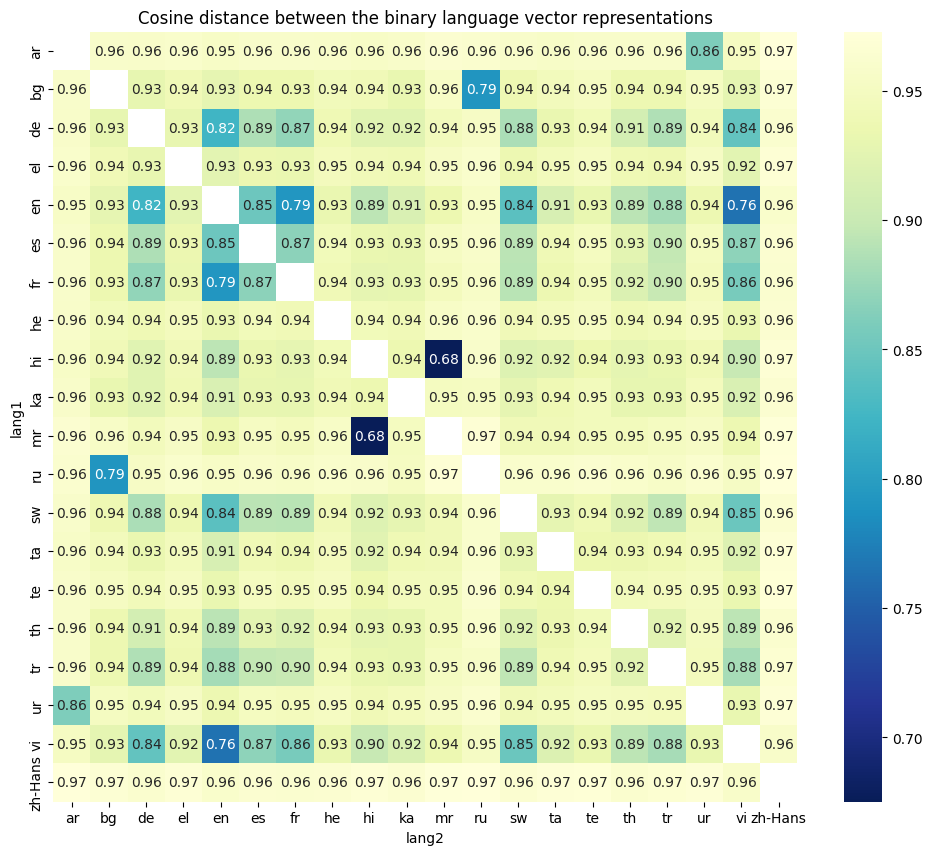
\includegraphics[width=0.5\textwidth]{img/chung_distances.png}
    \caption{Cosine distances between the language vectors $\vec{v}^l$ for Chung et al.}
    \label{fig:chung_distances}
\end{figure}

\begin{figure}[h]
    \centering
    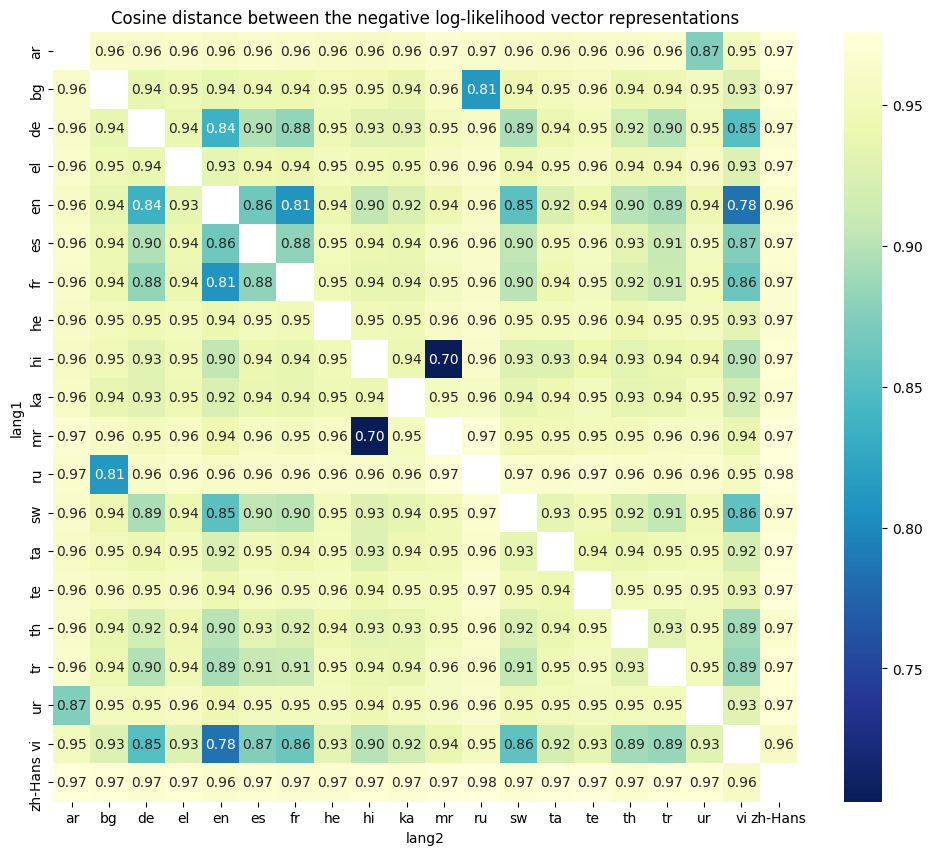
\includegraphics[width=0.5\textwidth]{img/liang_cosine_distances.png}
    \caption{Cosine distances between the language vectors $\vec{v}^l$ for Liang et al.}
    \label{fig:liang_cosine_distances}
\end{figure}

\begin{figure}[h]
    \centering
    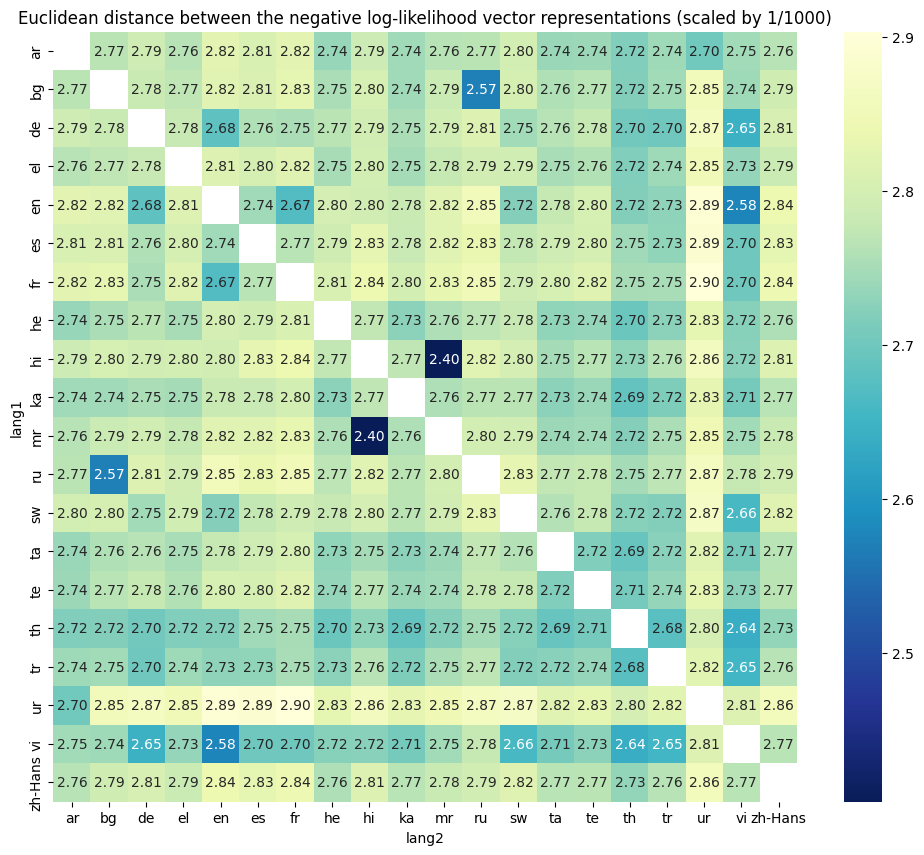
\includegraphics[width=0.5\textwidth]{img/liang_euclid_distances.png}
    \caption{Euclidean distances between the language vectors $\vec{v}^l$ for Liang et al.}
    \label{fig:liang_euclid_distances}
\end{figure}


With the vector representations $\vec{v}^l$ we can cluster the languages into $k$ clusters $C^k$ using the k-means algorithm. We use the implementation from \cite{scikit-learn} with the default parameters \xxx{check the parameters}. By normalizing the language representation vectors to unit length, we effectively switch to the cosine distance as the metric for the k-means algorithm. We experiment with $k \in \{4, 8, 12, 16, 20\}$. Note that $k=20$ corresponds to separating each language into a separate cluster which is similar to the method \textsc{TokMix} we introduce in \citet{limisiewicz_tokenization_2023}. 

Then, given a clustering of languages $C$, for each cluster $c_j \in C$ we create new training corpus by concatenating all of the pretraining data belonging to the cluster\footnote{Here we have departed slightly from the recipe in the papers and used 1M lines per language instead of using the pretraining data. The reasoning is that we know that 1M lines per language is enough data to train the tokenizers effectively and at the same time we do not run into out-of-memory problems. On the other hand we have effectively used more balanced data to train the cluster tokenizers than Chung and Liang did. The difference is best illustrated by considering the marginal case of number of clusters $k=1$. With one cluster we would effectively train the tokenizer on the balanced multilingual dataset ($\alpha = 0$) as opposed to the original papers where in the case of $k=1$ the tokenizer would be trained on the pretraining data where the language imbalance is present ($\alpha = 0.5$).}. We run the Sentencepiece algorithm again on these clustered corpora to arrive at cluster-specific vocabularies $V^{c_j}$. The vocabulary size for each cluster is determined following the Chung and Liang methods. For both methods we want to arrive at the final size of 120k tokens after merging the cluster-specific vocabularies. Therefore we need to determine the size of each cluster vocabulary $|V^{c_j}|$ such that $\sum_{j=1}^k |V^{c_j}| = 120k$. Moreover, we would like to distribute the capacity of the final vocabulary effectively so that each cluster is assigned enough tokens to cover the languages it contains. The Chung method sets the size of the cluster vocabulary to be proportional to the the size of the union over the monolignual vocabularies $|\bigcup_{l \in c_j} V^l|$ to determine the size of each cluster vocabulary $|V^{c_j}| = \frac{|\bigcup_{l \in c_j} V^l|}{\sum_{i=1}^k |\bigcup_{l' \in c_i} V^{l'}|} \cdot 120k$.

The Liang method sets the size of the cluster vocabulary to be proportional to the sum of the vocabulary allocations from \citet{zheng_allocating_2021} for the languages belonging to the cluster. We use the statistics from Table 9 in \citet{zheng_allocating_2021}, following \citet{liang_xlm-v_2023}.

After the tokenizers are trained, we merge the vocabularies using the method described in \xxx{ref}. 

Here we slightly improve the methods of Chung and Liang. By following the original method as described above, the final size of the vocabulary will be lower than the target we set. This is because the cluster vocabularies $V^{c_j}$ will contain overlapping tokens and merging will remove these duplicates. This negative effect becomes larger with the increasing number of clusters $k$. Therefore, on top of training the prescribed cluster vocabulary of size $|V^{c_j}|$, we also train slightly larger vocabularies $V_q^{c_j'}$ of size $|V_q^{c_j}| = q|V^{c_j}|$ for $q = 1.1, 1.2, 1.3$. We then select the minimum $q$ that results in a vocabulary of size at least 120k tokens after merging the cluster vocabularies. After that we trim the vocabulary if needed. This improvement is done to ensure the final vocabulary size is exactly 120k tokens and the comparison between the methods is fair.

The resulting clusters and the corresponding per-cluster vocabulary sizes are found in Table \xxx{todo add table}

\subsection{Reproducing the \textsc{VoCap} method}

%     - Zheng
%         - train monolingual tokenizers for all 20 languages with vocab sizes 1k ... 40k
%         - load a sample of CC100 data for each language (50k lines per language)
%         - tokenize the data with all of the monolingual tokenizers
%         - compute the ALP for each language and vocabulary size
%         - select the best vocabulary size for each language greedily
%         - we also experiment with optimizing CPT instead of ALP
%         - we also experiment with computing the CPT improvement on each merge step instead of precomputing it for all vocab sizes

%         - they have this suspicious plot with ALP with Joint250k, Joint500k and VoCap500k and the differences are too much

From the high level, the \textsc{VoCap} method works by selecting the best vocabulary size for each language and then merging the monolingual vocabularies. The best vocabulary size is determined by maximizing the overall \textit{Average Log Probability} metric defined in \xxx{ref}. 

To replicate the \textsc{VoCap} method, we first need to compute the \textsc{ALP} metric for each language and each vocabulary size. We therefore train monolingual tokenizers using Sentencepiece with default settings for all 20 languages with vocabulary sizes from 1k to 40k.\footnote{The more effective way, not discussed by \citet{zheng_allocating_2021}, would be to modify the Sentencepiece unigram trainer code to produce a tokenizer after each prune iteration. That way we would get series of tokenizers with decreasing vocabulary size in one go, instead of running the trainer 40 times. As the computational cost of training the tokenizers is not high, we have not implemented this improvement.} We use 1M lines per language for training the monolingual tokenizers again, following \citet{zheng_allocating_2021}. Note that for Chinese the tokenizer vocabulary size starts at 5k due to the large number of unique logograms in the language. 

% reference for 1M lines: https://github.com/bozheng-hit/VoCapXLM/blob/main/train_mono_spm.py#L73

We then load a sample of CC100 data for each language (100k lines per language) and tokenize each monolingual corpus with the respective tokenizers of increasing vocabulary sizes. We are then able to compute the $\mathrm{ALP}(l, V)$ \xxx{fix the formula so that it matches related work} for each language $l$ and each vocabulary size $V \in \{1000, 2000, ..., 40\,000\}$

Now we can greedily select the best vocabulary sizes. We start with selecting the lowest vocabulary size for each language (1k for all languages except Chinese where we start with 5k). We merge the selected vocabularies of the tokenizers. Then in each iteration, we check which language would benefit the most from increasing the vocabulary size by 1000. Concretely, we check the increase in ALP for each language and increase the vocabulary size for that language by merging the bigger vocabulary with the total vocabulary. We repeat this process until the total vocabulary size reaches 120k tokens. Any tokens over the limit are removed from the vocabulary.

Contrary to \citet{zheng_allocating_2021}, we do not use the $\beta$ rescaling factor to account for the pretraining corpus size. By setting $\beta$ to 0, we want to achieve the best ALP for each language regardless of their corpus size. This is because we want to balance the low-resource languages, not necessarily achieve the best performance on the downstram tasks.

The final vocabulary sizes for each language are found in Table \xxx{todo add table}.

Additionally, we also experiment with optimizing the \textsc{CPT} metric instead of \textsc{ALP}. We also experiment with computing the \textsc{CPT} improvement on each merge step instead of precomputing it for all vocab sizes, since the metric increase might be slightly different for the intermediate tokenizer. None of these modifications lead to substantially better results and so we stick to the original method. \xxx{rewrite this or remove it}

\subsection{Merging the tokenizers}

%     - merging the tokenizers
%         - merging is not really described in the papers
%         - of course we take the union of the vocabularies
%         - but how to set the logits?
%             - to illustrate that even this step should be documented, the probabilities of XLM-V vocabulary do not sum to one
%     - reaching the target size
%         - train +10\%, +20\% of the target size and then prune

For all reproduced methods, the last step is to take several UnigramLM tokenizers and merge them into the final, multilingual tokenizer. Now we will describe how do we merge tokenizers in our case. Unfortunately, the merging step is not described fully in any of the reproduced papers. In the case of the UnigramLM tokenizers, tokenizer $\tau$ consists of vocabulary (set of strings) $T^\tau \subset \Sigma^\star$ and the corresponding logits $L^\tau: \Sigma^\star \rightarrow \mathbb{R}$ so that $\sum_{t \in T^\tau} \exp(L^\tau(t)) = 1$. \xxx{maybe mention the logits in related work} The logits are used for finding the most probable segmentation of an input sentence. 

To create the merged vocabulary for input tokenizers $\tau_1, ... \tau_m$ we take the union over the vocabularies:

\begin{equation}
    T^\tau \coloneqq \bigcup_{i=1}^m T^{\tau_i}
\end{equation}

We set the merged logits to the log of the average probability of the token in the input tokenizers:

\begin{equation}
    \forall t \in T^\tau: L^\tau(t) \coloneqq \log(\frac{1}{m} \sum_{i, t \in T^{\tau_i}} \exp(L^{\tau_i}))
\end{equation}

If the token $t$ is not present in some of the input tokenizers, we consider the probability of the token for that tokenizer to be zero. 

In this way the sum of the probabilities of the tokens in the merged vocabulary is one and thus the merged tokenizer is a valid UnigramLM tokenizer. We can see this by the following derivation:

\begin{equation}
    \sum_{t \in T^\tau} \exp(L^\tau(t)) = \sum_{t \in T^\tau} \frac{1}{m} \sum_{i, t \in T^{\tau_i}} \exp(L^{\tau_i}) = \frac{1}{m} \sum_{i=1}^m \sum_{t \in T^{\tau_i}} \exp(L^{\tau_i}) = \frac{1}{m} \sum_{i=1}^m 1 = 1
\end{equation}

\xxx{the second equality should be maybe more explained}

We argue that this is the most natural way to merge the tokenizers and so we assume this is probably the way the other authors did the merging. By observing the logits in the tokenizer released by \citet{liang_xlm-v_2023} though, we see that the authors do merge the logits in some way but the sum of the probabilities in the final tokenizer is $\approx 4.55$ (not counting the special tokens), which suggests some problems in the merging step.

\xxx{We have also checked empirically, that the individual tokenizers perform similarly to the merged tokenizer and so the merging procedure seems to preserve the properties of the merged tokenizers.}

% urls for the tokenizers:
% https://github.com/bozheng-hit/VoCapXLM/blob/main/VoCap_500k/sentencepiece.bpe.model
% https://huggingface.co/facebook/xlm-v-base/blob/main/sentencepiece.bpe.model


\section{Proposed methods}

% - motivation for word-balancing:
%     - we assume that there is a topic imbalance in the CC100 corpus
%         - assume there is 99% of news and 1% biology
%         - the name of the ministry of agriculture will be more common than the word "evolution"
%             - but it is more useful to cover the most common words in biology than the uncommon words in news
%         - by balancing the words we may achieve better coverage of the topics
%     - we assume it is better to split roots of words and not have many inflected forms of the same word
%         - if the word "evolution" occurs much more frequently than "evoluce", the model might learn "evolution" but will oversegment "evoluce"
%         - by balancing the words we may arrive at a better segmentation because it will be more useful to split "evolution" into evolu + tion and evoluce into evolu + ce

We propose to compare the replicated methods with the original method from \citet{conneau_unsupervised_2020} with $\alpha=0.3$. Moreover, we also propose to simply use the balancing factor $\alpha=0.0$, which leads to data balance, that is equal in the number of lines across all languages. 
Specifically, both methods use the same Sentencepiece tokenizer implementation as used in the replications. We use the Unigram LM as in \citet{conneau_unsupervised_2020}, set the vocabulary size to 120k and leave the rest of the parameters default. The main difference is the training data where $\alpha=0.0$ uses 1M lines per language and $alpha=0.3$ uses a sample of 10M lines from the CC100 with the language balance factor $\alpha=0.3$. 

% The next method we propose is based 

\section{Model pretraining}

With the tokenizers replicated and trained, we will train the language models to be able to assess the influence of the tokenization method on the language model performance.

We use the Huggingface framework \cite{wolf_transformers_2020} for pretraining the language model. We use the example script from the Huggingface repository to pretrain the language model with the Masked Language Model objective. The model architecture is based on a scaled-down version of XLM-R\textsubscript{Base} \cite{conneau_unsupervised_2020}. The size of embeddings is kept at 768, the number of attention layers is reduced from 12 to 8, the number of attention heads is reduced from 12 to 6. The maximum sequence length is set to 128 tokens. The vocabulary size is 120\,000. The total number of parameters is roughly two times smaller than the original XLM-R\textsubscript{Base}.

The models are pretrained for 10k steps with batchsize 8192 achieved by using gradient accumulation. This amounts to $\approx 1.6$ epochs over the training dataset. The learning scheduler is linear with warmup for the first 500 steps. The learning rate is set to $5e-4$

\section{Model probing}

- technical details

% Model
% - mBERT - 120k vocabulary, 12-layer, 768-hidden, 12-heads, 110M parameters
